\chapter{Introduction}

Climate change mitigation policies aimed at reducing the long-term costs of fossil-based electricity generation are driving the growth of renewable energy resources. An important consequence of the transition from fossil to renewable resources is that the marginal cost of energy is more often near zero. Low marginal cost energy has important consequences throughout the electric system and industry because it changes the assumptions on which existing markets and regulations operate. Low marginal cost energy diminishes the effectiveness of energy markets, particularly in regions where wind and solar have significant energy and capacity potential. 

Extensive analysis has been dedicated to understanding the impact of increasing supply intermittency arising from growing use of renewable generation resources. Unpredictable ramping durations and magnitudes have significant implications for energy market designs. But market mechanisms for scheduling and dispatching renewable resources in wholesale markets remain largely focused on discovery of the increasingly irrelevant marginal cost of energy, rather than the emerging marginal cost of ramping resources that support renewable energy resource integration. As more renewable resources enter the generation portfolio, market designs predicated upon coordination using market-clearing prices for energy will perform poorly because they do not take full account of all the different marginal costs involved in offering and dispatching units from distributed heterogeneous technologies. In particular, increasing distributed energy resources (DERs) shifts relative cost away from the marginal cost of energy, and toward the time cost of capacity, energy storage, and ramping resources needed to fulfill contractual commitments.

Changes in the electricity resource portfolio are causing changes in the relative values of different resource capabilities. Flexibility as a general capability has risen in relative importance with the growth in DERs and their heterogeneity. Examples of flexibility include dispatchability (can the resource be called on for energy or grid services?) and ramping rate (how quickly can the resource deliver energy or grid services?). Digital interconnection and automation increase the range of dispatchability in the resource portfolio, making more resources (including DERs) more flexible and thus more potentially valuable. The ramping rate, and particularly resources which can ramp quickly, increases flexibility by increasing the amount of DERs the distribution system can absorb. Fast-ramping resources have value because they can offset energy imbalances and provide both energy and grid services to maintain system balance. Moreover, some DER technologies are fast ramping. As DERs proliferate, electricity market designs will have to adjust to the increasing relative value of flexibility. The price may often be the marginal cost of ramping rather than the marginal cost of energy.

Despite market design challenges, the combination of environmental policy and falling production costs has driven a proliferation of distributed energy resources in electric power systems. Transactive energy is emerging as a fundamentally new market-based approach to coordinating electric energy delivery in systems with very high levels of DERs. Transactive energy combines technology and engineering with market design and economic principles. Autonomous device response to informative, emergent prices is the hallmark of transactive energy.  

\section{Background}

Transactive energy was originally conceived of as \textit{transactive control} to address the problem of optimally integrating large numbers of small resources into electric power system operations. Transactive control provided a mechanism at the retail level, without requiring large amounts of potentially private information about those resources' supply and demand functions, such as would be required for a formal numerical optimization solution.  This problem became more prominent as utilities struggled to integrate a growing variety of behind-the-meter energy resources, including energy efficiency, demand-side-management, demand response, photovoltaics, electrification, and energy storage into their system operations.  These resources have widely varying supply and demand functions in a context in which prices can change in near-real time, and can be automated to self-dispatch based on a complex mix of energy, capacity, and ramping prices.

Transactive energy synthesizes the technologies and control theory from engineering with the market design and institutional theory from economics into a cyber-physical-social system. Digital technologies create the possibility of energy devices changing their settings autonomously in response to prices, and control theory provides a framework for modeling, testing, and understanding the individual and system effects of such capabilities. Economics provides the institutional framework in which the rules by which those outcomes emerge are embedded. That institutional framework is the price system and market processes. Prices which emerge from market interactions communicate information about the underlying subjective preferences and opportunity costs of resource and device owners. By responding to those prices through their devices' algorithms, market participants coordinate with each other, especially as the relative scarcity of energy and system resources change in real time. Markets are information generation and communication processes that lead to decentralized coordination.

An essential feature of the economics of transactive energy is that people are individually distinct, with personal, subjective preferences over the goods and services they consume. As producers their perceptions of the opportunity costs they face are also subjective. Knowledge of these preferences and opportunity costs is private and not available to others. A price system operating within a clear set of rules provides a decentralized mechanism for gathering information and learning about these preferences and opportunity costs, even among strangers (or their devices). The market process of mutual learning and decision-making enables prices to emerge that coordinate the actions and plans of all users of the system.

The initial objective of using transactive energy was to mitigate local system capacity constraints. The Olympic \cite{hammerstrom2007} and Columbus \cite{widergren2014} projects achieved this objective within 5 minutes of a constraint's emergence. As market-based solutions to the distributed resource dispatch problem, these demonstrations became canonical models for the kind of Pareto-optimal\footnote{Pareto optimality is based on an economic efficiency concept whereby a change from one outcome to another is deemed \textit{Pareto efficient} if it makes some people better off without making any worse off. A Pareto optimal system is one in which no participant can be made better off without making another participant worse off.} solution that transactive energy systems provide in general.

All the supply resources in the Olympic and Columbus tests had non-trivial energy cost functions and relatively trivial cost functions with respect to flexibility services, because at the time the question of flexibility with high DER penetration had not yet achieved its current prominence.  Concern has grown recently that transactive control systems will be less effective at optimally dispatching modern distributed resources because so many resources now have zero or nearly zero marginal energy costs, or have no obvious energy cost function at all, yet they have non-trivial impacts on bulk system capacity and ramping behavior that affects system reliability and resilience. Transactive systems designed around the marginal cost of energy no longer create and communicate information that is as useful for system coordination as in the past. 

The energy-centric focus of wholesale power markets limits our ability to develop a more comprehensive approach to designing and deploying transactive systems that can accommodate all relevant types of prices and support the long-term financial demands of the parties to such a system. The long-term objective of TESS is to address this challenge and provide a platform that supports the path from the present-day energy-centric market paradigm to one that supports the full panoply of DER capabilities that are plausible in a well-developed, economically sustainable, reliable, and customer-focused transactive system.

\subsection{History}

Transactive energy builds on earlier work to understand the effects of communicating timely information using prices on individuals and on systems. Fred Schweppe and his students at MIT \cite{schweppe1978} published the earliest work on price-based coordination in power systems in the late 1970s.  They envisioned a system in which energy prices expressed when and where significant constraints on the system were present. They envisioned using those prices to signal appropriate responses by energy producers and consumers. Among other things, their work led to the development of the modern wholesale energy market design now widely used in liberalized energy systems around the world. This work was the origin of security-constrained economic dispatch (SCED); such price-based dispatch is an antecedent to transactive energy.

However, the wave of market liberalization that swept over bulk power systems never reached the same heights at the retail level.  A combination of strong consumer-advocacy, regulatory reticence, and a lack of understanding of consumer behavior has severely limited retail market liberalization.  In regions where retail liberalization proceedings are active (e.g., Texas, New York, Illinois), it has been dominated by financial and scheduling opportunities rather than addressing the dispatch and control challenges in distribution operations when significant DER is present.

A number of efforts to solve the problem of price-based dispatch for retail-side resources were reported over the intervening years.  Huberman et al. \cite{huberman1991} demonstrated using price signals to control building HVAC systems.  Later, and more or less simultaneously Hammerstrom et al. \cite{hammerstrom2007} and Kok et al. \cite{kok2013} demonstrated a more comprehensive retail dispatch system involving not just thermal loads, but also distributed generation, appliances, and industrial loads to manage a feeder constraint.  Finally, Widergren et al. \cite{widergren2014} further expanded on the approach by demonstrating a multi-feeder system with an integrated control-room interface to manage and coordinate the system in real time, as well as an integrated billing and settlement system. Other more recent North American pilot projects in California, New York, and Maine are discussed in a recent SEPA report \cite{sepa2019}.

The concepts present in these systems form the basis of all modern transactive energy systems.  The technical details of any given transactive system may vary, but the fundamental notions, mechanisms, and operational characteristics remain largely consistent with the Olympic, Columbus, and PowerMatcher model with variations to suit the particulars of utilities, resources, and wholesale market designs.

\subsection{Economic Foundations}

%this may not be the right place to put this but we need an economic theory section

Transactive energy synthesizes the technologies and control theory from engineering with the market design and institutional theory from economics into a cyber-physical-social system. Digital technologies create the possibility of energy devices changing their settings autonomously in response to prices, and control theory provides a framework for modeling, testing, and understanding the individual and system effects of such capabilities. 

Economics provides the institutional framework, the rules by which those outcomes emerge. That institutional framework is the price system and market processes. Prices that emerge from market interactions communicate information about the underlying subjective preferences and opportunity costs of resource and device owners. By responding to those prices through their devices' algorithms, market participants coordinate with each other, especially as the relative scarcity of energy and system resources change in real time and capabilities such as flexibility change in relative value. Markets are information generation and communication processes that lead to decentralized coordination.

\subsection{Technical Foundations}

The Olympic and Columbus projects both used a simple 5-minute double auction as the market design that enabled the energy price at which supply equalled demand to emerge.  During the time interval leading up to the auction clearing, all active resources autonomously submitted a reservation price for a time-invariant power capacity over the upcoming operating interval. Resources with available supply submitted offers for a power supply at a reservation price, and end-use consumption resources submitted asks for a a power demand at a reservation prices. Reservation prices reflect the subjective preferences and subjective perception of opportunity costs of the resource owners. When the market cleared, the clearing price was delivered to all devices that submitted bids, and devices were dispatched based on the relationship between the clearing price and their original bids. Loads consumed if the clearing price was less than or equal to their offer price, and generators produced if the clearing price was greater than or equal to their offer price.

The specific bidding strategies employed by loads and distributed generators were idiosyncratic according to the peculiarities of the resource in question.  In general thermostatic loads used a user-specified comfort price curve to convert between temperature and price. Users chose the balance between temperature and price based on their personal, subjective preferences. Other resources such as municipal water storage pumps used similar strategies where the function was controlled by the owner of the resource. Resources where the thermostat could not be directly controlled, such as water heaters used alternate strategies such as probabilistic load shedding strategy with no asking bid at all.  In the case of asynchronous back-up generators, the resources bid as loads with asking prices that accounted for licensed run-hours, start-up costs, and minimum run-time requirements.

The transactive systems all relied on automation to ensure that devices submitted truthful bids and responded as expected to clearing prices.  In that sense, the devices could be relied upon to operate truthfully in the short term.  Even so, a number of technical issues arose.

\begin{enumerate}
    
    \item The auction mechanism needed to know the state of all loads, including those unresponsive loads that were not participating in the dispatch mechanism.  To compute the total unresponsive load, all transactive loads submitted a current state along with the ask/offer and quantity.  The market estimated the unresponsive load by deducting the total bid load that was on from the measured load at the constrained point.  The accuracy of this mechanism was critical to computing accurate prices and ultimately to achieving the constraint management objective.  Although the mechanism was not perfect, the approach worked well enough to also account for losses on the system.

    \item The system relied on all devices to dispatch accurately immediately after receiving the clearing price. However, some devices could not maintain the required dispatch for the full five minutes.  For instance, thermostatic loads that respond to price changes with temperature set-point adjustments would sometimes change state before the market interval elapsed. These behaviors resulted in deviations from the power equilibrium computed by the auction. Some projects explored solutions to this problem and provided some measure of relief.  For example, Chassin \cite{chassin2015} presented thermostat lockouts lasting the same duration as the market, and the Columbus project used bidding strategies the compensated for expected early state change.
    
    \item The real-time pricing mechanisms presented a number of challenges that were only partially addressed by the demonstration projects.  First, all loads in the residences were subject to the real-time price, including all the unresponsive loads.  This generally did not present a problem to consumers provided they were made aware when prices were very high.  In the Olympic project, both thermostats and white-good appliances provided a high-price warning, but the 5-minute time-step was not practical for general demand response, especially when customers could not observe the signal and no advance warning was available.  
    \\~\\
    Second, the fact that scarcity rents arose more frequently on congested feeders gave rise to the potential for widely varying costs according to customer location on the feeder, which was viewed as an unfair cross-subsidy from the constrained feeders to the rest of the system.  To mitigate this effect, a month-end rebate mechanism was introduced. But this rebate essentially undid the fundamental design principle of the real-time price mechanism insofar as any short-term price exposure the customer experienced was effectively mitigated by the rebate in the long term. There was no mechanism to commit the scarcity rents to directly mitigating the constrained resources.
    
\end{enumerate}

The bill settlement systems in the Olympic and Columbus project were quite different.  The Olympic project was designed as a classical economic experiment.  Consequently, participants were given an initial endowment, and their account balances were charged based on when they used energy. Using energy during low-price periods resulted in smaller charges against the endowment than in high-price periods. At the end of each quarter, the participants received the remaining balance as a cash payment. Customers continued to pay their normal utility bill under their current tariff and as a result, there was a potential for interactions between the side-payments and the energy bills.  Another difficulty with this approach was the need to compute an appropriate initial endowment for each customer.  A baseline energy demand model was used to compute the expected demand, which presented a number of technical challenges that were addressed with only moderate success.  Overall, these difficulties did not have a significant adverse effect on the experiment itself. However, it is clearly not well-suited to a more general system and presents many of the same difficulties demand response aggregators face today with other mechanisms to induce and reward good demand response behavior.

In the Columbus project settlement was integrated into the utility's billing system under a tariff designed specifically for the project and approved by the regulatory authority. While this is much more akin to how utilities might normally approach such matters, it was much more difficult to design, approve, and implement than the side-payment mechanism used in the Olympic project.  However, the tariff mechanism did not suffer from the baseline model problems experienced in the Olympic experiment.

Finally, all the devices were reprogrammed to provide the desired response capabilities. In the case of residential thermostats, a vendor was hired to provide the needed thermostats.  In both cases, there were inherent limitations that made the behavior of the thermostats less than ideal. Nevertheless, the thermostats worked well enough to provide ample demand response capabilities during peak load periods.  In the case of commercial building HVAC, distributed generators, and the municipal water pumps, the control system were reprogrammed to work directly with agents that handled bidding and response on their behalf.

\subsection{Current Challenges}

The TESS system will be developed and deployed in a staged approach to enable the shortest possible time-to-market, while laying the foundations for the full system.  The first version of TESS is considered a minimum viable product (MVP), based almost entirely on the existing technology, assets, and methods available at the present time. For this reason, the MVP will have limited benefits when compared to the full range of benefits possible using future versions.  But the MVP will be developed and deployed in such a manner that forward compatibility with the future versions is maximized.

The experience gained from transactive system paradigms that have been proven in the field suggest a number of outstanding technical challenges that TESS must address in the MVP.  

\begin{description}

    \item[Financing:] Financing the deployment of transactive systems was not considered in the Olympic and Columbus demonstration projects. Although transactive systems can generally pay for themselves, the financial returns may not be fast enough to meet the expectations of typical customer or utility financing sources. 
    \\~\\
    \textit{Projects require financing mechanisms that support longer term paybacks often found in transactive systems.}

    \item[Engineering Tools:] The engineering design methodology for a transactive system is more complex that the engineering design methods normally required for utility project planning.  
    \\~\\
    \textit{Projects require a new suite of engineering design tools that facilitate the planning and operation of transactive systems.}

    \item[End-use Control Automation:] The vast majority of end-uses that can theoretically participate successfully in transactive system lack the control and communications infrastructure required to do so practically. Most of the existing end-use load control capabilities are proprietary and intrinsically limited to the scope of the program(s) they support rather than offering customers the opportunity and flexibility to benefit from all possible stream of revenue that transactive system can reveal.  
    \\~\\
    \textit{Projects require a systematic and open program to support and encourage the integration of new and existing behind-the-meter resources .}

    \item[Control Room Operations:] Distribution system planners and operators lack the tools and training to design and operate transactive systems. Transactive systems have fundamentally different characteristics and operate using a different paradigm, which can often seem opaque and non-intuitive to a well-trained power system engineer.  
    \\~\\
    \textit{Projects require a comprehensive program to train utility planners and operators to use a standard suite of tools.} 

    \item[Billing System Integration:] Adapting an existing utility metering and billing infrastructure is a significant barrier to adoption of a transactive solution.  The rate at which transactions occur, the complex mix of prices and quantities, and the bandwidth limitations of automated metering infrastructure (AMI) can make deployment of a transactive system cost-prohibitive or outright impossible using existing the back-office infrastructure typically found in utility operations. These systems were simply not designed to perform the functions required by a transactive system.  
    \\~\\
    \textit{Projects require a new payment infrastructure that is shared by both utilities and customers.}

\end{description}

\subsection{Technology Readiness}

The TESS research program divides transactive technologies into two basic categories: (1) Mature Technologies, and (2) Developmental Technologies.  Mature technologies have been proven to meet certain operational requirements, albeit with assumptions and constraints that are likely to limit the broad applicability.  Development Technologies lack the maturity necessary to be utilized reliably in an operational settings.

The US Department of Energy uses a grading system called the Technology Readiness Level (TRL) to represent the relative maturity of energy system technologies \cite{DOE-G413-2009}. For transactive systems, we propose the TRL scale be defined as follows.

\begin{enumerate}

    \item[\footnotesize TRL0] \textbf{Unsolved problem}: This represents a technology that has yet to be identified to address an existing problem.
    
    Supporting information includes a statement of the problem or challenge to be addressed, with possible literature review and technology assessment to support the motivation need for basic research to solve the problem.
    
    \item[\footnotesize TRL1] \textbf{Basic principles observed and reported}: This is the lowest level of technology readiness. Scientific, engineering, and economic research begins to be translated into applied R\&D. Examples might include paper studies of a technology's basic properties or experimental work that consists mainly of observations of existing systems. 
    
    Supporting information includes published research or other references that identify the principles that underlie the technology.

    \item[\footnotesize TRL2] \textbf{Technology concept and/or application formulated}: Once basic principles are observed, practical applications are proposed. Applications are speculative, and there may be no proof or detailed analysis to support the assumptions. Examples are still limited to analytic and simulation studies. 
    
    Supporting information includes publications or other references that outline the applications being considered and that provide analysis to support the concepts. The step up from TRL1 to TRL2 moves the ideas from pure to applied research. Most of the work is analytical, numerical, or paper studies with the emphasis on understanding the science better. Experimental work is designed to corroborate the basic scientific observations made during TRL1 work.
    
    \item[\footnotesize TRL3] \textbf{Analytical and experimental critical function and/or characteristic proof of concept}: Active research and development (R\&D) is initiated. This includes analytical and simulation studies and laboratory-scale studies to physically validate their predictions for independent elements of the technology. Examples include components that are not yet integrated or representative tested with simulations or emulators. 
    
    Supporting information includes results of laboratory tests performed to measure parameters of interest and comparisons to analytical predictions for critical subsystems. At TRL3 the work has moved beyond the paper phase to experimental work that verifies that the concept works as expected in simulation environments. Components of the technology are validated, but there is no attempt to integrate the components into a complete system. Modeling and simulation is often used to complement physical experiments.
    
    \item[\footnotesize TRL4] \textbf{Component and/or system validation in laboratory environment}: The basic technological components are integrated to establish that the constituents will work together in a system. This is relatively ``low fidelity'' when compared with the eventual system. Examples include integration of ad hoc hardware in a laboratory and testing with a range of software simulators and hardware emulators and small scale tests on actual systems. 
    
    Supporting information includes the results of the integrated experiments and estimates of how the experimental components and experimental test results differ from the expected system performance goals. TRL4-6 represent the bridge from scientific research to engineering. TRL4 is the first step in determining whether the individual components will work together as a system. The laboratory system will probably be a mix of on hand equipment and a few special purpose components that may require special handling, calibration, or alignment to get them to function.
    
    \item[\footnotesize TRL5] \textbf{Laboratory scale, similar system validation in relevant environment}: The basic technological components are integrated so that the system configuration is similar to (matches) the final application in almost all respects. Examples include testing a high-fidelity, laboratory scale system in a simulated environment with a range of simulations, emulations, and actual systems. 
    
    Supporting information includes results from the laboratory scale testing, analysis of the differences between the laboratory and eventual operating system/environment, and analysis of what the experimental results mean for the eventual operating system/environment. The major difference between TRL4 and TRL5 is the increase in the fidelity of the system and environment to the actual application. The system tested is almost prototypical.
    
    \item[\footnotesize TRL6] \textbf{Engineering/pilot-scale, similar (prototypical) system validation in relevant environment}: Engineering-scale models or prototypes are tested in a relevant environment. This represents a major step up in a technology's demonstrated readiness. Examples include testing an engineering scale prototypical system with a range of systems. 
    
    Supporting information includes results from the engineering scale testing and analysis of the differences between the engineering scale, prototypical system/environment, and analysis of what the experimental results mean for the eventual operating system/environment. TRL6 begins true engineering development of the technology as an operational system. The major difference between TRL5 and TRL6 is the step up from laboratory scale to engineering scale and the determination of scaling factors that will enable design of the operational system. The prototype should be capable of performing all the functions that will be required of the operational system. The operating environment for the testing should closely represent the actual operating environment.
    
    \item[\footnotesize TRL7] \textbf{Full-scale, similar (prototypical) system demonstrated in relevant environment}: This represents a major step up from TRL6, requiring demonstration of an actual system prototype in a relevant environment. Examples include testing full-scale prototype in the field with a range of systems in a limited range of real-world conditions. 
    
    Supporting information includes results from the full-scale testing and analysis of the differences between the test environment, and analysis of what the experimental results mean for the eventual operating system/environment. Final design is virtually complete.
    
    \item[\footnotesize TRL8] \textbf{Actual system completed and qualified through test and demonstration}: The technology has been proven to work in its final form and under expected conditions. In almost all cases, this TRL represents the end of true system development. Examples include developmental testing and evaluation of the system in the full range of real-world conditions. 
    
    Supporting information includes operational procedures and training systems that are virtually complete. An Operational Readiness Review (ORR) has been successfully completed prior to the start of hot testing.
    
    \item[\footnotesize TRL9] \textbf{Actual system operated over the full range of expected conditions}: The technology is in its final form and operated under the full range of operating conditions. Examples include using the actual system with the full range of real-world conditions.
    
    Supporting information includes an ongoing record of performance issues, problem diagnosis and remedies, a record of user training, and end-user support.
    
\end{enumerate}

\subsubsection{Mature Technologies}

This section outlines the existing technologies that have matured sufficiently (e.g., TRL6) to be included in the minimum viable product that will be deployment in the first operational system.

\begin{description}

    \item[Centralized retail capacity double auction] (TRL6): The technology needed to deploy a centralized retail capacity double auction was originally developed by PNNL for the Olympic pilot project. It was subsequently deployed in an improved form by Battelle in the Columbus pilot project. Variants of the same technology have piloted by others, such as PowerMatcher.
    
    \item[Automated bidding] (TRL6): Automated bidding strategies for residential and commercial building thermostats, a limited number of white good appliances, distributed generators, and municipal water pumps were piloted in the Olympic project.  Thermostats have been piloted in other projects since, e.g., Columbus, PowerMatcher.  Other automated bidding strategies have yet to be piloted in a utility-integrated transactive system and therefore have lower TRLs, e.g., residential rooftop photo-voltaics (TRL1), vehicle and battery chargers (TRL3), commercial building central plants (TRL5). 
    
    \item[Automated response] (TRL6): Automated price response technology usually has at least the same level of maturity as Automated Bidding technology. In some cases Automated Response technologies have already been piloted while the corresponding bidding strategies have not, e.g., residential hot water heaters (automated bidding is TRL4) and dryers (automated bidding is TRL3).
    
    \item[Centralized side payment settlement] (TRL6): In the Olympic pilot centralized side payments were used to conduct the economic experiment and a side-payment settlement system was deployed to support that mechanism.
    
    \item[Integrated billing] (TRL6): In the Columbus pilot a utility-integrated billing system was used to settle the transactive payments under a regulator-approved tariff.
    
    \item[Control room systems] (TRL6): In the Columbus pilot, a control room display with inputs to adjust the feeder constraints was deployed.
    
\end{description}

\subsubsection{Developmental Technologies}

This section outlines the requirements for a full-fledged transactive system that have not yet been developed or full demonstrated in operational environment, or are not sufficient mature to be included in the minimum viable product.

\begin{description}

    \item[Decentralized identity management] (TRL0): A mechanism to manage and use secure transactive device identities is needed.  There is a proposed GMLC project (BLOSEM) that will develop and pilot this technology, but the basic principles have yet to be reported.

    \item[Decentralized double auctions] (TRL0): Centralized double auction are easy to deploy and operate and have been piloted already. There is economic theory to suggest that using decentralized double auctions presents a number of significant scaling and operational advantages. At the present time, there is no report of a functional concept for how to implement decentralized auction mechanisms in an operational transactive utility environment.

    \item[Centralized retail energy storage double auction] (TRL0): The mechanism to operate an energy storage price discovery mechanism has not been proposed yet.

    \item[Proof of control] (TRL1): A concept for the basic principles of ``proof-of-control'' mechanisms have been reported.  A mechanism that demonstrates whether devices perform as required with meter-grade measurement for a transactive system has yet to be demonstrated and reported. 
    
    \item[Centralized retail ramping response double auction] (TRL1): The mechanism to operate a ramping response price discovery mechanism has been notionally proposed, although it has not been report yet.

    \item[Real-time orderbook] (TRL2): Orderbook technology used in many other market environment offer the opportunity to dispatch resources in real-time rather than periodically using double auctions.  The basic principles of orderbook technology has been initially studied in work at SLAC as part of the ``PowerNet with Market'' project for the California Energy Commission's Advanced Simulation Program\footnote{``Powernet with Markets'' is funded by the California Energy Commission under CEC Grant EPC-15-043.}.

    \item[Payments for data-sharing] (TRL3): A proof of concept of CleanCoin was completed by students at Carnegie Mellon University in the fall of 2018. The system has not been reported.

    \item[Operator training system] (TRL3): The utility operators of transactive systems will require training to manage the utility infrastructure required to engage transactive resources both at the retail and wholesale level.  A SLAC research project has reported analytic and experimental evidence to support the critical functions in a proof-of-concept for operator training \cite{hu2019}. 

    \item[Decentralized settlement] (TRL5): Centralized billing and payment systems are typically simple to implement, provided a third-party is available to mediate the payments.  In the case of centralized billing systems, the utility transaction settlements must feed into the existing utility billing system, which can be a significant barrier to adoption for transactive energy system.  Decentralized settlement and payment system bypass the utility billing system and avoid the need for a third-party to mediate payments. This technology has been proposed for transactive energy systems, and some pilots have been completed using price-responsive resources, but a completely decentralized transactive settlement system that include bidding, measurement, and payment has not been reported in the literature at this time. There are however a number of systems (e.g., LO3, OmegaGrid) that demonstrate the technology elements required for a pilot of a fully transactive double auction-based capacity dispatch system.

\end{description}

\section{TESS Program Life-Cycle}

A proposed transactive energy system program must undergo a thorough process of evaluation, development, and deployment to be successful in operations.  This process is illustrated in Figure~\ref{fig:tess_program_elements}.
\begin{figure}[!t]
    \centerline { \scalebox{0.5} { \xymatrix {
        (1)~Development
    &
    &   (2)~Deployment
    &
    &   (3)~Operations
    \\       
    &
    &   
    &
    &   *++[F]{Scheduling}
    \\      
    &   *++[F]{Financing}   \ar[r]
    &   *++[F]{Outreach}    \ar[r]
    &   *++[F]{Provision}   \ar`r[ru][ru] \ar`r[rd][rd]
    &
    \\  *++[F]{Screening}   \ar`r[ru][ru] \ar`r[rd][rd] \ar`r[rru][rru] \ar`r[rrd][rrd] \ar`r[rrru][rrru] \ar`r[rrrd][rrrd]
    &
    &
    &
    &   *++[F]{Operations}
    \\
    &   *++[F]{Engineering}      \ar[r]
    &   *++[F]{Install}     \ar[r]
    &   *++[F]{Bootstrap}   \ar`r[ru][ru] \ar`r[rd][rd]
    \\
    &   \qquad \qquad \qquad
    &
    &   \qquad \qquad \qquad
    &   *++[F]{Settlement}
    \save "1,1"."6,2"*++[F--]\frm{}\restore
    \save "1,3"."6,4"*++[F--]\frm{}\restore
    \save "1,5"."6,5"*++[F--]\frm{}\restore
    }}}
    \caption{TESS program elements}
    \label{fig:tess_program_elements}
\end{figure}
The program development (Stage 1) focuses on the resource screening, program financing, and engineering design for deployment (Stage 2).  During deployment, customers and resources are identified and made ready for operations (Stage 3).  Once operations are started, scheduling, dispatching, and settlement is run continuously according to the program design parameters developed in Stage 2. This section discusses the details of the program elements in each phase.

\subsection{Program Development}

The first stage of the program life-cycle is \textit{program development}. During this stage potential programs are screened and evaluated for their financing potential.  Program options that pass initial screening would be developed during the engineering design process. During program development the following resources would be considered.

\begin{description}

    \item[Energy Efficiency (EE):] EE measures typically focus on improving the overall energy performance of a home.  As a general rule, EE measures reduce both the peak and total energy use, which can have significant impact on load growth. But these measures can also improve the benefits of demand-side management and demand-response measures by lengthening the natural period and/or broadening the duty-cycle range of a home's heating/cooling systems. 

    \item[Demand-side Management (DSM):] DSM focuses on replacement of older, less-efficient electric equipment such as a heating/cooling equipment, refrigerators, and freezers.  Sometimes replacement of older white-goods appliance are included if the energy or power demand improvement is beneficial to both the utility and the customer. DSM programs offer many of the same benefits as EE measures. But DSM programs also afford the consumer an opportunity to install equipment and appliances that include load control capabilities that can help achieve some transactive energy benefits.

    \item[Demand Response (DR):] DR systems enable direct load control from remote systems such as utility load-shedding programs and demand response aggregators.  Direct load control technology is a transitional capability on the path to a fully transactive system.  Direct load control technology allows utilities and aggregators to shed, shift, shape or shimmy loads according to a utility's operating objectives and the customers' willingness to participate.

    \item[Photovoltaics (PV):] PV system provide utilities with a local source of renewable energy that can reduce midday peak loads and reduce system losses.  When combined with other resources such as DR and energy storage, PV resources can be very effective in reducing utility costs, provided the coordination of these resources is performed well.

    \item[End-use electrification (EV):] End-use electrification resources generally focus on electric vehicle chargers because their impact on the utility's infrastructure can be very significant relative to other end-use electrification.  However, all fossil-based end-uses should be considered in an electrification program evaluation, including space and water heating, cooking, and clothes drying. The benefit of end-use electrification are twofold: (1) a greater share of the customer's load is electric, which permits a greater diversity of resources to participate in the transactive energy system, and (2) the overall increased electric demand supports the utility's long-term growth and near-term transition to an economically viable transactive energy system.

    \item[Energy Storage (ES):] ES resources can greatly magnify the benefit of PV and EV resources by allowing surplus energy production in the midday to be stored and then released during the evening hours when overall load peaks.  The combination of DR, PV, EV, and ES is particularly potent and transactive energy systems offer a mechanism to more easily realize their full joint potential.

\end{description}

\subsubsection{Screening}

Program screening is the process of identifying whether a particular combination of transactive resources yields financial and other benefits to both the utility and its customers, whether the utility and its customers would benefit from simultaneous investment in other resources, such as a fiber to the premises network for broadband, and whether the combination of programs is financially viable, as shown in Figure~\ref{fig:impact_analysis}.
\begin{figure}[!t]
    \centerline { \scalebox{0.72} { \xymatrix {
    &
    &
    &
    &   *++[F]{EE~Impacts}
    \\  *++[F]{Customer~characteristics} \ar`r[ddr]`[ddrr][ddrr]
    &
    &
    &
    &   *++[F]{DSM~Impacts}
    \\  *++[F]{Wholesale~history} \ar`r[dr]`[drr][drr]
    &
    &
    &
    &   *++[F]{DR~Impacts}
    \\  *++[F]{Load~history} \ar[rr]
    &
    &   *++[F]{Analysis} \ar`r[ruuu]`[ruuur][ruuur] \ar`r[ruu]`[ruur][ruur] \ar`r[ru]`[rur][rur] \ar[rr] \ar`r[rd]`[rdr][rdr] \ar`r[rdd]`[rddr][rddr] 
    &
    &   *++[F]{PV~Impacts}
    \\  *++[F]{Weather~assumptions} \ar`r[ur]`[urr][urr]
    &
    &
    &
    &   *++[F]{EV~Impacts}
    \\  *++[F]{Tariff~options} \ar`r[uur]`[uurr][uurr]
    &
    &
    &
    &   *++[F]{ES~Impacts}
    }}}
    \caption{Resource impacts analysis}
    \label{fig:impact_analysis}
\end{figure}
A number of program valuation analysis methods will be considered based on both finance and engineering simulation of the programs, as shown in Table~\ref{tab:screening}. 
\begin{table}[!t]
    \caption{Example screening options}
    \label{tab:screening}
    \centering
    ~\\
    \begin{tabular}{cllrc}
        \hline
        Option & Program & Profile & Net~benefit & \%~Positive
    \\  \hline \hline
        $[$X$]$ & EE && \$120/meter.y & 45\%
    \\  $[$~~$]$ & DSM && -- & --
    \\  $[$X$]$ & EV && \$120/meter.y & 55\%
    \\  $[$X$]$ & PV && \$450/meter.y & 90\%
    \\  $[$~~$]$ & DR && -- & --
    \\  $[$X$]$ & ES && \$25/meter.y & 10\%
    \\  \hline
    \end{tabular}
\end{table}
The simulations will allow consideration of both constructive and destructive interference between the resources, and express these as a correlation matrix to allow rapid evaluation of the ideal mix of programs. 

To evaluate the financial feasibility of the project, the screening process will consider a number of financial structures, ranging from traditional utility and customer debt to innovative combinations of debt, equity and catalytic philanthropic capital that are deployed in a special-purpose transactive energy entity that may also offer other services, such as broadband access. These innovative structures are an emerging financing mechanism to support infrastructure investments that provide a social good with a positive financial return, but have a long payback time. For each structure, the screening process will include an analysis of the financial performance for both the utility and their customers. Tables~\ref{tab:criteria1} and \ref{tab:criteria2} illustrate the performance of financing scenarios for the utility or transactive system operator, and their customers, respectively.  
\begin{table}[!t]
    \centering
    \caption{Example IRR analysis of financing scenarios.}
    \label{tab:criteria1}
    \includegraphics[width=\columnwidth]{tess_table_2.png}
\end{table}
\begin{table}[!t]
    \centering
    \caption{Example annual financial performance for the utility's customers}
    \label{tab:criteria2}
    \includegraphics[width=\columnwidth]{tess_table_3.png}
\end{table}
Equity IRRs are calculated over the ten-year project projections.  The 8\% IRR year is the year after final equity investment that the investment achieves an 8\% IRR. DSCR refers to the debt service coverage ratio, which reflects the ability of a project to pay its debt.

\subsubsection{Financing}

Financing is a critical process of a transactive energy system. Without financing the system cannot be deployed.  Financing options are evaluated in the screening, the project funding mechanism is selected, and the project is funded.  The mechanism by which the funds are brought into the project would depend on the expected performance of the project and the debt appetite of the utility and the utility's customers.  

Projects that are viable with traditional debt might be financed through traditional utility debt in combination with rate-basing the transactive energy system assets.  In this scenario, the utility customer's would self-finance the appropriate resources listed above.  

Alternatively, if a project is not viable with traditional utility debt, or a utility is unable to pursue such a debt scenario, a special purpose transactive energy entity can be created to offer transactive energy services to the utility by financing the customer-sited resources.  Such an entity would undertake operation of the transactive energy system or contract out to a transactive energy system specialist.  The entity can be financed with a mixture of debt, equity and catalytic philanthropic capital. It can be a subsidiary of the utility, a joint venture with the utility, or a stand-alone entity created by the equity investors. The entity can also own and/or operate other services for the community, such as fiber-optic based broadband.  

\subsubsection{Design}

A TESS program design involves selecting the types of resources that will be included in the schedule, dispatch, and settlement operations, and how many customers will participate using the selected resources. This analysis is performed using a series of simulations that quantifies the benefits and uncertainties associated with each program options as the number of customers changes. The analysis then computes the optimal balance of customers required to maximize the total system benefits.

The approach used is based on portfolio theory, as shown in Figure~\ref{fig:portfolio}. 
\begin{figure}[!t]
    \centering
    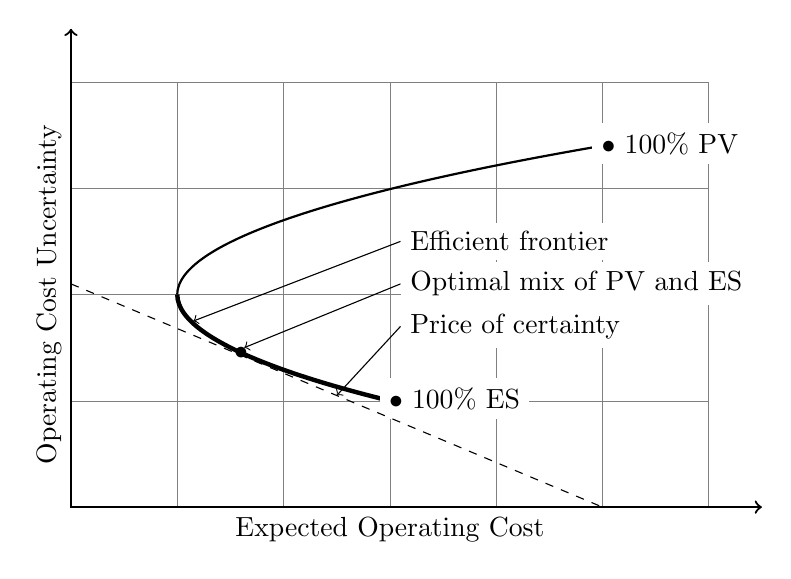
\begin{tikzpicture}[scale=1.35]
        % axes and grid
        \draw [very thin,gray,step=1] (0,0) grid (6,4);
        \draw [thick,<->] (0,4.5)--(0,0)--(6.5,0);
        \node [anchor=north] at (3,0) {Expected Operating Cost};
        \node [anchor=south,rotate=90] at (0,2) {Operating Cost Uncertainty};
        % curve
        \draw [ultra thick,rotate=90] (2,-1) parabola (1,-3);
        \draw [thick,rotate=-90] (-2,1) parabola (-3.4,5);
        \node [right,fill=white] at (2.9,1.02) {$\bullet$~100\% ES};
        \node [right,fill=white] at (4.9,3.42) {$\bullet$~100\% PV};
        % cost
        \draw [dashed] (0,2.1) -- (5,0); \node at (1.6,1.45) {$\bullet$};
        \draw [<-] (1.15,1.75) -- (3.1,2.5); \node [right,fill=white] at (3.1,2.5) {Efficient frontier};
        \draw [<-] (1.63,1.50) -- (3.1,2.1); \node [right,fill=white] at (3.1,2.1) {Optimal mix of PV and ES};
        \draw [<-] (2.5,1.05) -- (3.1,1.7); \node [right,fill=white] at (3.1,1.7) {Price of certainty};
    \end{tikzpicture}
    \caption{Example portfolio analysis for PV and ES customer resources}
    \label{fig:portfolio}
\end{figure}
Each customer resource has an associated expected cost impact and cost uncertainty resulting from its operation as a transactive resource.  When two different resource types are combined, their joint uncertainty varies according to the interactions between them, and the resulting impact on costs as a function of uncertainty follows a quadratic mix, as shown in Figure~\ref{fig:portfolio}. Only mixtures ``inside'' the curve are feasible, and given an arbitrary mixture no utility would choose to operate with a greater cost or uncertainty.  

Because it is a utility's objective to reduce both cost and uncertainty, the lower segment of the curve is the desired range of program subscriptions. This segment is referred to as the ``efficient frontier''.  Only mixtures participants with resource mixtures in this region of the feasible space would normally be selected. If the utility has an understanding of the value of certainty in the wholesale market, it is possible to identify a single point along the efficient frontier where mixtures of customer resources will minimize the joint cost and uncertainty. The design tools provide the simulation and analytic framework from which this result is obtained.

\subsection{System Deployment}

The goal of system deployment is to functionally integrate customer resources with utility systems such that the utility can leverage the combined resource flexibility in the bulk system scheduling operations.

\subsubsection{Outreach}

Outreach activities identify and contact consumers who own or control resources that can provide value-added services either to the utility, or to other customers, or both. While screening identifies which resources should be considered, outreach identifies consumers who own or who could own or host those resources. Outreach activities are segmented according to  channels for accessing customers (e.g., digital media, traditional media, direct mail) as well as enrollment programs, registration systems, and applications that specifically target consumers with desired resources such as rooftop photo-voltaics, electric vehicle, or energy storage. 

\subsubsection{Provisioning}

TESS, and the MVP in particular, is designed to represent the entire system in a multi-plane system with three independent graphs, as shown in Figure~\ref{fig:planes}: 
\begin{figure}[!t]
    \centering
    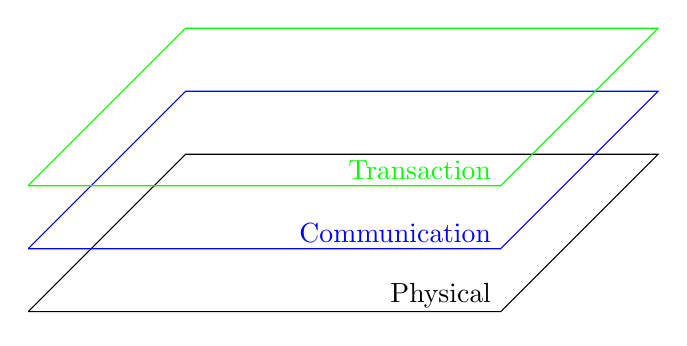
\begin{tikzpicture}[scale=2]
        \draw (0,0.0)--(1,1.0)--(4,1.0)--(3,0.0)--(0,0.0);
        \node [anchor=east] at (3,0.1) {Physical};
        \draw [blue] (0,0.4)--(1,1.4)--(4,1.4)--(3,0.4)--(0,0.4);
        \node [anchor=east,blue] at (3,0.5) {Communication};
        \draw [green] (0,0.8)--(1,1.8)--(4,1.8)--(3,0.8)--(0,0.8);
        \node [anchor=east,green] at (3,0.9) {Transaction};
    \end{tikzpicture}
    \caption{Multi-plane system structure}
    \label{fig:planes}
\end{figure}
1) the physical plane the represents system topology at an electrical level, 2) the communication plane that represents the information networks connecting various nodes, and 3) the transaction plane embodied in the blockchain network that facilitates the exchange of value between participants. Each plane captures specific information about the state of the system and can communicate it to other planes using protocols, some of which are current industry standards and others that need further development. For instance, the communications plane will use well established TCP/IP protocol whereas the transaction plane will use a yet-to-be-identified two-step consensus protocol that overcomes limitations of proof-of-work, the most commonly used distributed consensus protocol on several blockchains. 

Provisioning activities register users via apps and web portals as participants on the communications and transaction planes. This includes establishing an identity (private-public key pair) for each participant, updating information about controllable devices owned by each participant, installing apps to allow devices to place bids and respond to price changes, as well as allowing users to view wallet balance, receive tokens, spend tokens, etc. 

\subsubsection{Installation}

Installation activities simply include installing mobile apps (blockchain wallet, miners, and data collection app) on user's mobile devices, connect equipment, and ensure that price bid/response loops are closed correctly. TESS will use common application distribution platforms such as Apple App Store and Google Play Store to deploy it's suite of mobile apps.  

\subsubsection{Bootstrap}

Bootstrap solves the Cold Start Problem. At t=0, TESS has no data (labels, known outcomes, classes) available to make progress. To solve this, TESS tokenizes intrinsic value of data and offers tokens to early adopters who install TESS suite of applications and choose to share data streams such as electricity usage and urban mobility. Users trade authorizations for use of their data streams in exchange for tokens. Trades are managed through Smart Contracts deployed and executed on the Transaction plane of TESS. Note that this is the same token that will be used to trade value-add transactive services (such as ramping, energy etc.) on the network. 

The big question here, of course is, "how many tokens is the data worth?". This is the one of the core research problems we hope to address during the course of development. Our current thinking is to use bonding curve contract, commonly used in crypto-economics. A bonding curve is a mathematical curve that defines a relationship between price and token supply. A bonding curve contract is a specific type of contract that issues its own Continuous Token. Prices are continuously calculated by the contract based on a bonding curve that enables coordination of network participants to share data specific to a particular region or zip code. 

\subsection{System Operations}

The goal of system operations is to give the utility the operating tools needed to leverage the flexibility of customer resources in their bulk system operations by scheduling, dispatch, and settling retail-level transactions between themselves and their customers.

\subsubsection{Scheduling}

Scheduling operations relate to the utility's supply and demand for resources in the bulk system.  Specifically, utilities can trade their aggregated energy storage reserves, power capacity, and ramping rates in various wholesale markets or bilaterally with multiple counter-parties across the bulk power system.  

Most utilities already have bulk resource scheduling operations, so TESS is unlikely to offer significant changes to these systems unless it is adding a new market interface that did not previously exist.  However, TESS does need to provide the utility with a system to quantify and cost the availability of energy, power, and ramping resources through the TESS system as the basis for the bonding curves.  The TESS scheduling system provides a basic interface for the traders to schedule TESS resources in the bulk markets.

\subsubsection{Dispatch}

Dispatch operations give the utilities control over supply and demand for resources within its own distribution system.  Utilities can use TESS to manage the state of TESS energy, power, and ramping resources. Quantities and prices can be monitored to provide an indication of whether sufficient resources are available locally to maintain reliable and efficient system performance.  If resource shortfalls or surpluses emerge, these can be addresses through bulk system operations.

\subsubsection{Settlement}

Settlement operations handle both the short term token settlements and the long term pricing of tokens.  As resources trade tokens in the short term, the settlement system guarantees that tokens are exchanged among users and accounts remain balanced.  The settlement system using a blockchain to track token exchanges in an open ledger. Periodically, the token price is updated through reconciliation of energy, power, and ramping costs and revenues in the wholesale markets.

\section{Incremental Release Versions}

TESS will be deployed in multiple versions, with increasing capabilities becoming available in each update.  The first version will be the so-called ``minimum viable product'' (MVP), which is narrowly focused on capabilities which have been previously demonstrated or are considered absolutely necessary to any functional system.  The second version will address the real-time limitation of the MVP, and the third version will address the multi-price discovery limitations of the MVP.

\subsection{TESS Version 1 - Minimum Viable Product}

The first version of TESS will support the following capabilities.

\begin{description}

    \item[Periodic Double Auction] A five-minute retail real-time price double-auction was originally developed and deployed in the Olympic project and enhanced in the Columbus project. This auction mechanism will be supported in the MVP at arbitrary points in radial systems, and for arbitrary time intervals.
    
    \item[Capacity Pricing] Capacity pricing is a well-understood market mechanism for managing local constraints in distribution system.  The price has units of ``\$/MWh'' and is uniform within each time interval.
    
    \item[Thermostatic Loads] Auction bidding and price response will be supported for a limited set of smart-thermostats using a comfort-economy input from the consumer \cite{hammerstrom2007}.
    
    \item[Battery Storage] Auction bidding and price response will be supported for a limited set of battery storage systems using a reliability-economy input from the consumer.
    
    \item[Rooftop Photovoltaic] Auction bidding and price response will be supported for a limited set of rooftop photovoltaic system using a revenue maximizing strategy.
    
    \item[Electric Vehicle Chargers] Auction bidding and price response will be support for a limited set of EV chargers using a cost minimizing V1G strategy \cite{behboodi2016}.
    
    \item[Real-time Token Settlement] Token exchanges will be tracked and settled in a single blockchain for each utility's TESS operations.
    
    \item[Two-stage Token Pricing] Tokens will be priced periodically based on a wholesale operations settlement.
    
    \item[Consumer Experience Mobility] A mobile app will be deployed for customers to manage all their TESS comfort, reliability, and economy settings, as well as their account balance in one place.

    \item[Open Source/Open API] An open API will be deployed, and all the capabilities of the TESS 1.0 will be released as open-source code.
        
\end{description}

\subsection{TESS Version 2 - Real-time Markets}

In addition to the MVP capabilities, the second release of TESS will support a real-time orderbook. The most significant aspect of this change is that there is not longer a single market clearing interval. Instead devices immediately receive a price for market orders, and can commit resources for a wide range of times using limit orders. This gives the system much greater flexibility and decreases the minimum response time when a significant constraint or opportunity arises.

\subsection{TESS Version 3 - Multi-service Markets}

In addition to the TESS 2.0 capabilities, the third release of TESS will support storage and ramping pricing, as well as dispatch-to-schedule optimization of the utility's operations. This will give the system the ability to allocate the amount of energy stored by sending price signals that encourage or discourage energy storage according to system conditions.  The system will also have the ability to directly allocate the amount of ramping by sending prices signals that encourage or discourage ramping response according to system conditions.  Most importantly, the system will allocate these new resources such that the primary business objective, e.g., cost minimization, surplus maximization is satisfied optimally.

\section{Conclusions}

TESS is a platform to support the full business life-cycle of Transactive Energy Service Systems.  TESS supports the design, deployment, and operation of peer-to-peer trading to help utilities and their customers achieve efficient and resilient integration of distributed energy resources.  The TESS system contributes to the decarbonization and democratization of our energy infrastructure, while ensuring utilities sustain financial performance, engage their customers, and help support bulk power system reliability.

TESS is an open project. The research and development agenda, the production schedule, and the initial operations are conducted in a collaborative environment. Utilities, equipment vendors, funding agencies, and consumer groups are invited to participate in the development, deployment, and operation of TESS by contacting the Principal Investigators at SLAC National Accelerator Laboratory or the Program Manager at the US Department of Energy's Office Electricity.